
\begin{center}
    \vspace{5cm}
    {\Huge\textbf{\section{\underline{Docket}}}} % Large and bold text
    \begin{figure}[h]
        \centering
        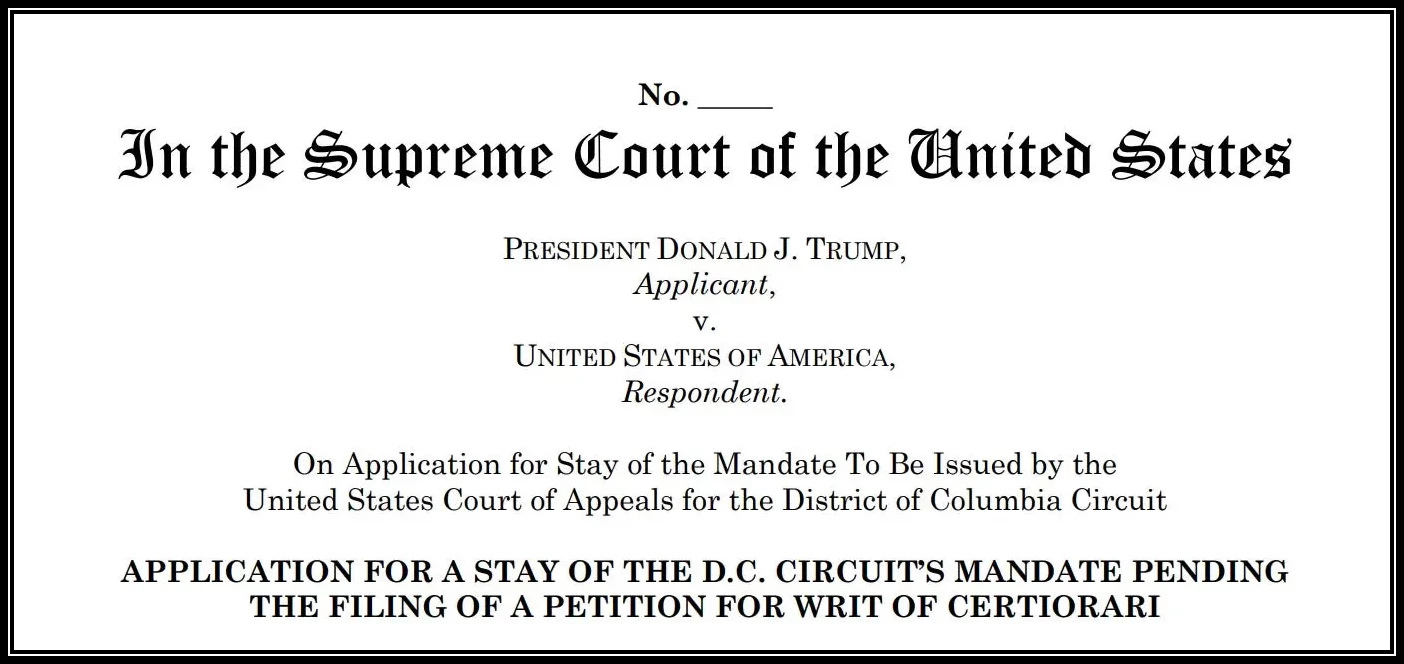
\includegraphics[width=0.85\textwidth]{Figures/intro_page_images/docket_filing.jpg} \\
        \footnotesize{Photo Credit: Chris Geidner (Law Dork)} \\
        \vspace{2mm}
        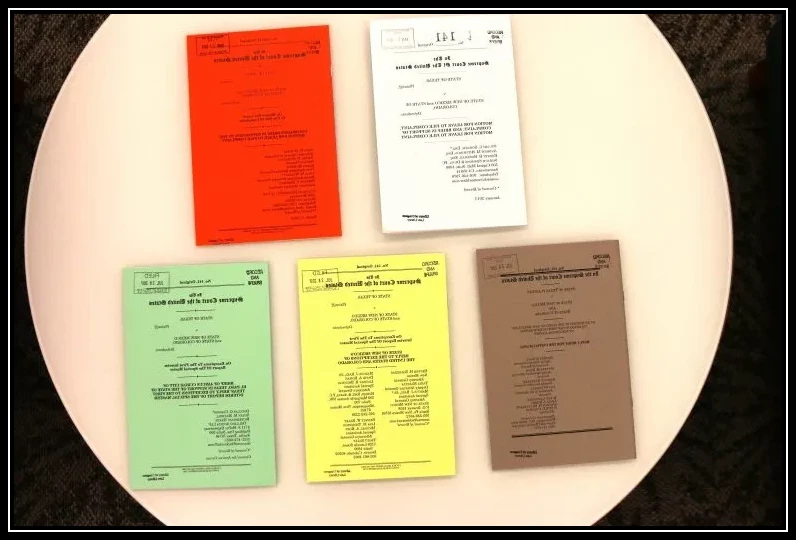
\includegraphics[width=0.85\textwidth]{Figures/intro_page_images/docket_filing_books.jpg} \\
        \footnotesize{Photo Credit: Donna Sokol (Library of Congress Blogs)} \\
    \end{figure}
\end{center}

\newpage

\begin{center}

\begin{table}[H]
    \centering
    \caption{What's Included (Docket)}
    \label{tab:example}
    \vspace{1mm}
    \begin{tabularx}{\textwidth}{>{\centering\arraybackslash}p{0.33\textwidth}>{\centering\arraybackslash}X}
        \toprule
        Topic & Description \\
        \midrule
        Filing Trends & \RaggedRight Filing trends of Applications, Motions, and Petitions (Non-Original Jurisdiction) by month (2023 Filing Term) and Year (2018 to 2023 Filing Terms). \\
        \addlinespace
        Courts of Origin & \RaggedRight Volume of petitions filed at the Court during the 2023 filing period by court of origin (e.g., U.S. Court of Appeals for the Fifth Circuit). Also an additional figure depicting the distribution of cases by Federal Appeals Circuit.  \\
        \addlinespace
        Amicus Curiae Briefs & \RaggedRight Average volume of amicus briefs filed in Granted petitions (2018 to 2023 Terms), as well as summary statistics of ``Cert'' (pre-grant) and ``Merits'' (post-grant) stage amicus filings for cases argued in the 2023 term. \\
        \bottomrule
    \end{tabularx}
\end{table}
\end{center}

\newpage
